\tp{\'Etude de l'�quilibre d'un solide soumis � l'action de 3 forces}

\section{Montage}
Soit le dispositif suivant :

\begin{multicols}{2}

\begin{center}
\begin{figure}[H]
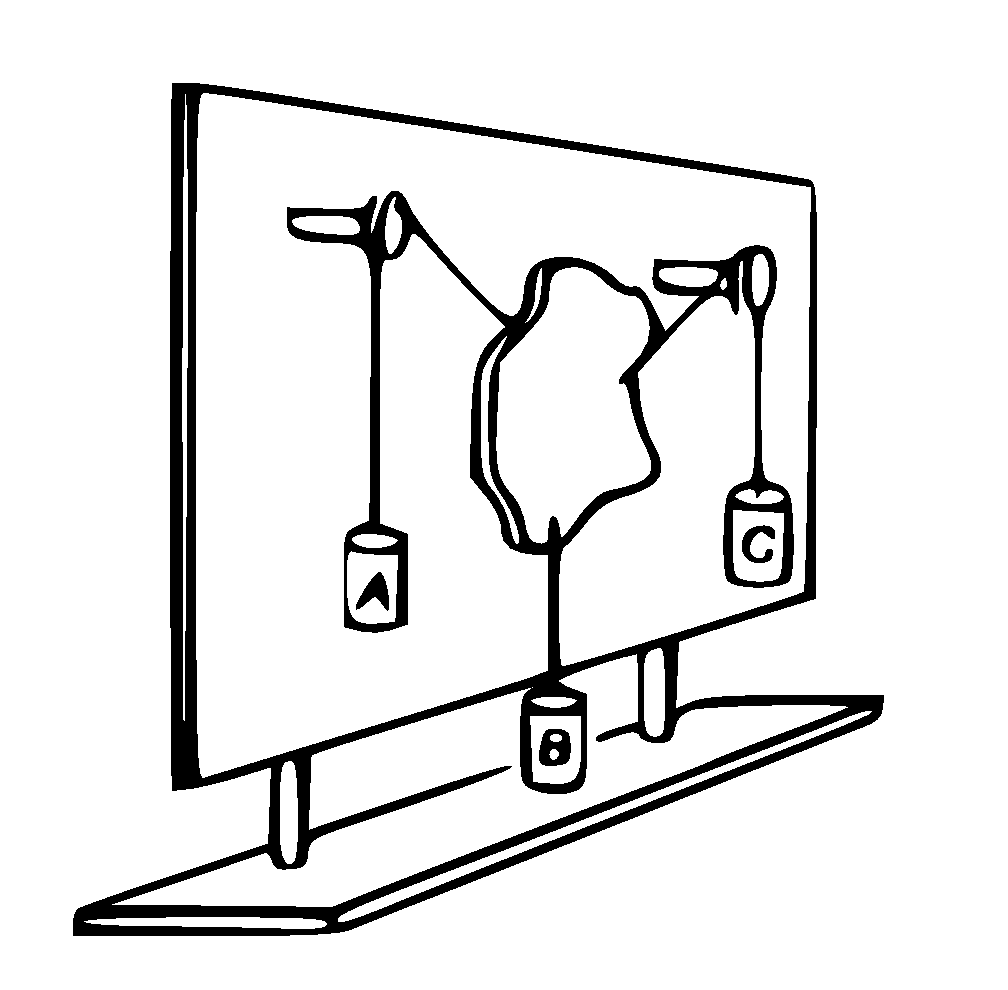
\includegraphics[width=6cm]{meca/tp_equilibre_solide_3_forces/montage_equi_3forces.eps}
\caption{Dispositif exp�rimental}
\end{figure}
\end{center}

% \begin{center}
% \begin{pspicture}(-3,-3)(3,3)
% \psgrid[subgriddiv=1,griddots=10]
% \pscircle(0,0){3}
% \pscircle*(0,0){0.1}
% \psline(-3,0)(3,0)

% \psline(0,3)(0,2.75)
% %\rotatebox

% \end{pspicture}
% \end{center}

\begin{center}
% D'apr�s http://melusine.eu.org/syracuse/pstricks/rapporteurs/fabrique/rml.tex
%\SpecialCoor

% \begin{pspicture}(-3,-3)(3,3)
% \pscircle{3}
% \pscircle[linestyle=dashed]{2.5}
% \pscircle[linestyle=dashed]{2}
% \pscircle[linestyle=dashed]{1.5}
% \pscircle[linestyle=dashed]{1}
% \pscircle[linestyle=dashed]{0.5}
% \psline(-3,0)(3,0)
% \pscircle*(0,0){0.1}
% \multido{\i=10+10}{36}{\psline(2.6;\i)(3;\i)} % grandes graduations(10�)
% \multido{\i=5+5}{72}{
%  \psline[linewidth=0.3\pslinewidth](2.8;\i)(3;\i)} % moyennes graduations (5�)
% \end{pspicture}

\begin{figure}[H]
\scalebox{1.414}{
\begin{pspicture}(-2,-2)(2,2)
\pscircle{2}
%\pscircle[linestyle=dashed]{2.5}
%\pscircle[linestyle=dashed]{2}
\pscircle[linestyle=dashed]{1.5}
\pscircle[linestyle=dashed]{1}
\pscircle[linestyle=dashed]{0.5}
\psline(-2,0)(2,0)
\pscircle*(0,0){0.1}
\multido{\i=10+10}{36}{\psline(1.6;\i)(2;\i)} % grandes graduations(10�)
\multido{\i=5+5}{72}{
 \psline[linewidth=0.3\pslinewidth](1.8;\i)(2;\i)} % moyennes graduations (5�)
\end{pspicture}
}

\caption{Rapporteur}
\end{figure}

\end{center}

\end{multicols}

\section{Mesures et interpr�tations}
\subsection{Masses $m_A$, $m_B$, $m_C$}
Soit les masses $m_A$, $m_B$, $m_C$ exer�ant des forces de traction sur les fils $A$, $B$,  $C$ et par suite sur le morceau de balsa ou polystyr�ne.


\noindent
$m_A$ = \troufixe{2cm} $kg$.\\
$m_B$ = \troufixe{2cm} $kg$.\\
$m_C$ = \troufixe{2cm} $kg$.


\subsection{Forces $P_A$, $P_B$, $P_C$ qu'exercent les fils $A$, $B$ et $C$ sur le morceau de balsa}
%Calculer les forces $P_A$, $P_B$, $P_C$ qu'exercent les fils $A$, $B$ et $C$ sur le morceau de balsa.

\noindent
$P_A$ = \troufixe{2cm} = \troufixe{2cm} $N$.\\
$P_B$ = \troufixe{2cm} = \troufixe{2cm} $N$.\\
$P_C$ = \troufixe{2cm} = \troufixe{2cm} $N$.



\subsection{Angles entre les directions des fils $A$, $B$ et $C$}

\noindent
$(A, B)$ = \troufixe{2cm} $�$.\\
$(B, C)$ = \troufixe{2cm} $�$.\\
$(C, A)$ = \troufixe{2cm} $�$.


\subsection{Interpr�tations}
\begin{enumerate}
\item Reporter les directions des fils � l'aide d'un rapporteur. Choisir une �chelle et tracer les forces $\vect{P_A}$, $\vect{P_B}$, $\vect{P_C}$. En utilisant la relation de Chasles, construire g�om�triquement $\vect{P_A} + \vect{P_B} + \vect{P_C}$. Que constatez-vous ?

\item \'Ecrire vectoriellement la condition d'�quilibre d'un solide soumis � l'action de 3 forces .

\cadre{1.2cm}

\end{enumerate}